\section{度量的构造}
\label{sec:metric-constructions}

第~\ref{chap:topological-spaces}章从已有空间构造了子空间、有限乘积和商空间，每次都规定了新空间的开集。有了距离以后，我们希望直接写出新空间的距离，并且让它诱导的拓扑恰好就是那里规定的拓扑。

本节逐项核对三种构造：把距离限制到子集，把各坐标的距离组合起来，以及先允许不同的点距离为零、再把这些点识别为一点。前两种对任意度量空间都可行；第三种只适用于由距离本身决定的识别，不能推广为任意商空间都有度量。

\subsection{子空间}
\label{sec:metric-subspace}

研究度量空间的一部分时，最直接的做法是保留原来的两点距离，只限制允许出现的点。

\begin{definition}[子空间度量]
\label{def:metric-subspace-metric}
设$(X,d)$是度量空间，$A\subseteq X$非空。限制$d_A=d|_{A\times A}$称为$A$上的\term{子空间度量}（subspace metric），$(A,d_A)$称为$X$的度量子空间。
\end{definition}

$A$中的点仍是$X$中的点，三条公理对$X$中任意点成立，自然对$A$中的点成立，所以$d_A$是度量。需要核对的是拓扑。$d_A$的开球是
\[
B_A(a,r)=\{y\in A:d(a,y)<r\}=B(a,r)\cap A,
\]
也就是环境中的球与$A$的交。

\begin{theorem}[子空间度量的拓扑]
\label{thm:metric-subspace-topology}
$d_A$诱导的拓扑等于$A$从$X$继承的子空间拓扑，即$V\subseteq A$在$(A,d_A)$中是开集，当且仅当存在$X$的开集$U$使$V=U\cap A$。
\end{theorem}

\begin{proof}
设$V$在$(A,d_A)$中是开集。对每个$a\in V$取$r_a>0$使$B_A(a,r_a)\subseteq V$，令$U=\bigcup_{a\in V}B(a,r_a)$。它是$X$的开集，并且
\[
U\cap A=\bigcup_{a\in V}\bigl(B(a,r_a)\cap A\bigr)=\bigcup_{a\in V}B_A(a,r_a)=V.
\]

反过来，设$U$是$X$的开集，$a\in U\cap A$。取$r>0$使$B(a,r)\subseteq U$，则$B_A(a,r)=B(a,r)\cap A\subseteq U\cap A$，所以$U\cap A$在$(A,d_A)$中是开集。
\end{proof}

于是第~\ref{chap:topological-spaces}章关于子空间的结论在度量子空间中都可以直接使用，只是开闭性要相对于$A$来判断。图~\ref{fig:metric-subspace-chord-arc}(a)是一个例子：在$\mathbb R$中取$A=[0,1]$，以$0$为中心、半径$1/2$的球在$A$中只剩$[0,1/2)$。

\begin{BookInlineFigure}
  \centering
  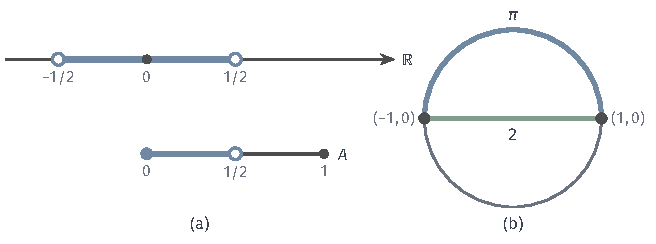
\includegraphics[width=111.1mm]{figures/04-spaces-measures-and-geometry/01-topology-and-metric/tikz/metric-subspace-chord-arc/figure.pdf}
  \caption{子空间的两个特点。(a)实轴上以$0$为中心、半径$1/2$的开球是$(-1/2,1/2)$，限制到$A=[0,1]$后成为$[0,1/2)$，它在$A$中是开集，在$\mathbb R$中不是。(b)单位圆周上，子空间度量量的是绿色弦长$2$，沿圆周的最短路径是蓝色半圆，长度$\pi$。}
  \label{fig:metric-subspace-chord-arc}
\end{BookInlineFigure}

这个集合可以写成$[0,1/2)=(-1/2,1/2)\cap A$，所以在$A$中是开集；$0$的左侧没有$A$的点，也就没有“越界”的点来破坏开性。再取$A=(0,1]$，它作为自身的子集总是闭集，但它在$\mathbb R$中不是闭集。环境决定了哪些点可以用来检验开闭。

子空间只保留环境中的两点距离，并不改用“沿着子集走”的距离。设$S^1=\{\bm x\in\mathbb R^2:\lVert\bm x\rVert_2=1\}$是单位圆周，如图~\ref{fig:metric-subspace-chord-arc}(b)所示，子空间度量下$(1,0)$与$(-1,0)$的距离是弦长$2$，而沿圆周走的最短长度是$\pi$。

弧长是圆周上另一个度量，它与弦长度量给出同样的拓扑，数值却不同。沿曲面或流形内部量出的路径长度需要切向量与长度的概念，在第~\ref{chap:riemannian-geometry}章建立。

\subsection{有限乘积空间}
\label{sec:metric-product}

几个度量空间的点组成坐标组时，需要一个距离同时比较各个坐标。设$(X_1,d_1),\ldots,(X_m,d_m)$是度量空间，$X=X_1\times\cdots\times X_m$，点记作$x=(x_1,\ldots,x_m)$。最常用的两种组合方式是求和与取最大：
\begin{equation}
\rho_1(x,y)=\sum_{i=1}^m d_i(x_i,y_i),\qquad
\rho_\infty(x,y)=\max_{1\leq i\leq m}d_i(x_i,y_i).
\label{eq:metric-product-metrics}
\end{equation}
这样定义的距离称为\term{乘积度量}（product metric）。$\mathbb R^2$上的$d_\infty$就是两个实轴的$\rho_\infty$。

两者都是度量。和或最大值为零，当且仅当每个$d_i(x_i,y_i)=0$，即每个坐标相同，这给出零距离判定；对称性逐坐标成立。三角不等式从每个坐标的不等式出发：
\[
d_i(x_i,z_i)\leq d_i(x_i,y_i)+d_i(y_i,z_i).
\]
对$\rho_1$，把这些不等式逐项相加。对$\rho_\infty$，右端两项分别不超过$\rho_\infty(x,y)$与$\rho_\infty(y,z)$，再对$i$取最大值。

两种度量还满足
\[
\rho_\infty\leq\rho_1\leq m\,\rho_\infty,
\]
因为$m$个非负数的和不小于其中最大的一个，也不超过最大者的$m$倍。图~\ref{fig:metric-ball-nesting}(b)画出了$m=2$时这组不等式对应的球的嵌套。与第~\ref{sec:metric-topology}小节的平面情形一样，它们的开球互相嵌套，诱导相同的拓扑。

\begin{theorem}[乘积度量的拓扑]
\label{thm:metric-product-topology}
$\rho_1$与$\rho_\infty$诱导的拓扑都等于第~\ref{chap:topological-spaces}章中$X_1,\ldots,X_m$的有限乘积拓扑。
\end{theorem}

\begin{proof}
由于两者诱导相同的拓扑，只需对$\rho_\infty$证明。乘积拓扑以形如$U_1\times\cdots\times U_m$（每个$U_i$是$X_i$的开集）的集合为基。最大值小于$r$等价于每个坐标距离都小于$r$，所以$\rho_\infty$的开球恰是
\[
B_{\rho_\infty}(x,r)=B_{d_1}(x_1,r)\times\cdots\times B_{d_m}(x_m,r).
\]
每个开球都是乘积拓扑的基元素，度量拓扑的开集都是乘积拓扑的开集。

反过来，设$x\in U_1\times\cdots\times U_m$。对每个$i$取$r_i>0$使$B_{d_i}(x_i,r_i)\subseteq U_i$，令$r=\min_i r_i$，则$B_{\rho_\infty}(x,r)\subseteq U_1\times\cdots\times U_m$。所以乘积拓扑的基元素在度量拓扑中也是开集。
\end{proof}

\begin{example}[两类坐标的乘积]
\label{ex:metric-product-two-coordinates}
取$X_1=\mathbb R$（通常距离）与$X_2=\{0,1\}^3$（Hamming距离），点$x=(0.2,010)$、$y=(0.5,011)$。实数坐标相差$0.3$，二进制串相差$1$位，于是
\[
\rho_1(x,y)=0.3+1=1.3,\qquad\rho_\infty(x,y)=\max\{0.3,1\}=1.
\]

在$\rho_\infty$下，$x$的半径$1/2$的球由第二坐标与$010$相同、第一坐标落在$(-0.3,0.7)$中的点组成：Hamming距离只取整数，要求它小于$1/2$就是要求两个串完全相同。
\end{example}

可见乘积距离小，意味着每个坐标都必须接近；哪个坐标先限制住球的形状，取决于各坐标距离的取值方式。

\subsection{伪度量}
\label{sec:metric-pseudometric}

有时我们只通过某些特征比较对象。比较平面上的点时如果只看横坐标，令
\begin{equation}
p(\bm x,\bm y)=\lvert x_1-y_1\rvert,
\label{eq:metric-first-coordinate-pseudometric}
\end{equation}
则$(0,0)$与$(0,5)$的“距离”为零，尽管它们是不同的点。$p$满足对称性和三角不等式，也满足$p(\bm x,\bm x)=0$，只缺零距离判定中“距离为零推出两点相同”这一半。

\begin{definition}[伪度量]
\label{def:metric-pseudometric}
设$X$非空。映射$p:X\times X\to[0,\infty)$若对任意$x,y,z\in X$满足$p(x,x)=0$、$p(x,y)=p(y,x)$与$p(x,z)\leq p(x,y)+p(y,z)$，则称$p$为$X$上的\term{伪度量}（pseudometric）。
\end{definition}

伪度量常由“忽略一部分信息”产生。向量空间上的\term{半范数}（seminorm）$\lVert\cdot\rVert$允许非零向量的长度为零，$p(\bm x,\bm y)=\lVert\bm x-\bm y\rVert$就是伪度量。第~\ref{chap:integration}章用积分比较函数时会遇到同样的情形：两个只在一个点上取值不同的函数，按积分算出的差异为零。

伪度量仍然有开球$B_p(x,r)=\{y:p(x,y)<r\}$。第~\ref{sec:metric-topology}小节证明开球构成拓扑基时，只用了“每点到自身距离为零”（使$x\in B(x,r)$）与三角不等式，没有用到“距离为零推出两点相同”。所以那里的论证逐字适用：伪度量的开球也生成一个拓扑，开集的球判据也相同。

这个拓扑不能区分零距离的点。在横坐标伪度量下，开球是一条竖直带形：
\[
B_p((0,0),1)=\{\bm x:\lvert x_1\rvert<1\},
\]
它同时包含$(0,0)$与$(0,5)$，见图~\ref{fig:metric-pseudometric-quotient}。一般地，若$p(x,y)=0$，则对任意$r>0$有$y\in B_p(x,r)$且$x\in B_p(y,r)$，于是$x$的每个开邻域都含有$y$，反之亦然。

所以只要存在不同的零距离点，伪度量拓扑就不满足Hausdorff条件。极限也随之不唯一：常值点列$(0,0),(0,0),\ldots$按$p$既趋于$(0,0)$，也趋于$(0,5)$。

\begin{BookInlineFigure}
  \centering
  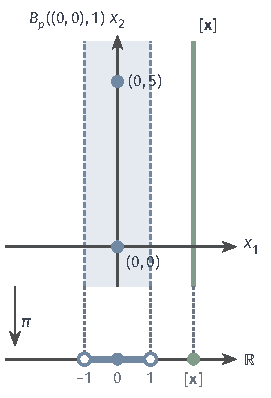
\includegraphics[width=45.903mm]{figures/04-spaces-measures-and-geometry/01-topology-and-metric/tikz/metric-pseudometric-quotient/figure.pdf}
  \caption{横坐标伪度量及其等价类。蓝色竖直带形是开球$B_p((0,0),1)$，点$(0,0)$与$(0,5)$同在其中，无法区分。绿色竖线是一个等价类$[\bm x]$。商映射$\pi$把每条竖线压成实轴上的一点，带形压成开区间$(-1,1)$。}
  \label{fig:metric-pseudometric-quotient}
\end{BookInlineFigure}

\subsection{零距离等价类上的度量}
\label{sec:metric-quotient}

既然伪度量无法区分零距离的点，自然的做法是把它们当成同一个点。下面验证这样做的每一步都合理，并说明得到的空间就是第~\ref{chap:topological-spaces}章意义下的商空间。

设$p$是$X$上的伪度量。规定$x\sim y$当且仅当$p(x,y)=0$。它是等价关系：自反性来自$p(x,x)=0$，对称性来自$p$的对称性，传递性来自
\[
p(x,z)\leq p(x,y)+p(y,z)=0.
\]
记$x$的等价类为$[x]$，商集为$X/{\sim}$，商映射为$\pi(x)=[x]$。

\begin{theorem}[零距离等价类上的度量]
\label{thm:metric-quotient-metric}
令$\hat d([x],[y])=p(x,y)$。则$\hat d$不依赖代表元的选取，是$X/{\sim}$上的度量，并且它诱导的拓扑等于$\pi$给出的商拓扑。
\end{theorem}

\begin{proof}
先证$\hat d$定义合理。设$x\sim x'$，$y\sim y'$。式~\eqref{eq:metric-reverse-triangle}的推导只用了对称性与三角不等式，所以对$p$也成立。于是
\[
\begin{aligned}
\lvert p(x,y)-p(x',y')\rvert
&\leq\lvert p(x,y)-p(x',y)\rvert+\lvert p(x',y)-p(x',y')\rvert\\
&\leq p(x,x')+p(y,y')=0.
\end{aligned}
\]

再核对公理。对称性与三角不等式从$p$继承。若$\hat d([x],[y])=0$，则$p(x,y)=0$，即$[x]=[y]$，零距离判定成立。

最后比较拓扑。由定义，$\pi$把$B_p(x,r)$映成$B_{\hat d}([x],r)$，并且
\[
\pi^{-1}\bigl(B_{\hat d}([x],r)\bigr)=B_p(x,r).
\]

设$V$在$\hat d$下是开集，$x\in\pi^{-1}(V)$。取$r$使$B_{\hat d}([x],r)\subseteq V$，则$B_p(x,r)\subseteq\pi^{-1}(V)$，所以$\pi^{-1}(V)$是$p$下的开集，$V$是商拓扑的开集。

反过来，设$\pi^{-1}(V)$是开集，$[x]\in V$。取$r$使$B_p(x,r)\subseteq\pi^{-1}(V)$，则$B_{\hat d}([x],r)=\pi(B_p(x,r))\subseteq V$，所以$V$在$\hat d$下是开集。
\end{proof}

回到横坐标伪度量。$(x_1,x_2)$的等价类是竖直线$\{x_1\}\times\mathbb R$，映射$[\bm x]\mapsto x_1$是$X/{\sim}$到$\mathbb R$的双射，并且
\[
\hat d([\bm x],[\bm y])=\lvert x_1-y_1\rvert.
\]
所以把零距离的点识别以后，得到的正是带通常距离的实轴：竖直方向的信息被丢掉，横坐标的距离被完整保留，这就是图~\ref{fig:metric-pseudometric-quotient}中从上到下的投影。

这一构造之所以可行，是因为等价关系由$p$自身给出，球在识别前后一一对应。对任意等价关系，商空间未必有度量。在$\mathbb R$上规定$x\approx y$当且仅当$x-y\in\mathbb Q$，考察商拓扑中的非空开集$U$。

$U$在$\mathbb R$中的原像是非空开集，含有某个区间$(a,b)$，又是若干等价类之并，因而含有$(a,b)+\mathbb Q=\mathbb R$。于是商拓扑只有空集和全集两个开集。商集有无穷多个点，两个不同的点不能用不交开集分开，按第~\ref{sec:metric-topology}小节的分离性，任何度量都不能诱导这个拓扑。
